%!TEX spellcheck
%!TEX root = ../bachelor_paper.tex
\documentclass[../bachelor_paper.tex]{subfiles}
\graphicspath{{\subfix{images/}}}
\begin{document}

\chapter{Results}
    \label{ch:res}
    
We were able to successfully generate performance profiles for the benchmarking workloads described in Section \ref{sec:bench/sum}. The workloads vary highly in instruction distribution, however for most of them, arithmetic instructions are the dominant instruction type overall (see Figure \ref{fig:res/overall/inst}). Exception to these rules are \texttt{embench edn}, \texttt{embench matmult int}, \texttt{embench nsichneu}, and \texttt{riscv vvadd} which favor load instructions; \texttt{embench statemate} which favors store instructions; as well as \texttt{riscv median} which favors branching instructions. As can be seen in Figure \ref{fig:res/overall/inst}, the difference between the most favored category and the runner up appears to be rather large on average. Indeed, the mean difference between the first two categories over all 39 workloads is 32.11\% points, where only 7 workloads have a disparity of less than 10\% points, with 25 having a disparity of over 20\% points and 17 having a disparity greater than the mean. This indicates that each workload strongly prefers one type of instruction with arithmetic instructions being the clear overall favorite. 

Moreover, we can see that almost no workload executed uses FPU instructions with \texttt{embench minver} being the only significant contender with a share of 13.8\%. Only \texttt{mibench-automotive susan} and \texttt{mibench-telecomm FFT} even register with a share of 0.21\% and 0.01\% respectively.

Not all workloads tested support hardware loops. Of those which do, most of them display vastly different \ac{HWL} utilization, depending on the algorithm implemented. Of special note is almost 75\% of workloads take more than 50\% of branches (see Figure \ref{fig:res/overall/branch_tk}). Given the \emph{branch not taken} approach taken in RI5CY, this incurs high branching penalties. However, it also indicates a loop-heavy algorithm. In fact, all five programs with a load coefficient less than 1 (meaning less instructions loaded from level 2 than executed) have a branch taken percentage well above 50\% (we intentionally excluded \texttt{tak} included in the \emph{custom} set here, as it only executes 2555 instructions is thus too small to draw conclusions from). 

The opposite conclusion is not possible however, as loop size also matters with regards to the harsh constraint of a 4 instruction prefetch buffer. \texttt{nettle aes} and \texttt{nettle sha256} have a branch taken rate of 53.68\% and 91.22\% as well as a fetch coefficient of 0.91 and 0.71 respectively. Meanwhile Dhrystone only managed a fetch coefficient of 1.39 with a branch taken rate of 64.89\%. In general, there are more instructions loaded into the prefetch buffer than are executed. Overall, for each instruction executed, about 1.17 instructions are fetched with a standard deviation of 0.2. As can be seen in Figure \ref{fig:res/overall/fetch_waste}, workloads loading less than 1 instruction per instruction executed are often significantly bellow this mark. Indeed the mean fetch coefficient for just them is only 0.84 with a standard deviation of only 0.09, indicating that these workloads use many short loops able to fit inside the prefetch buffer. Conversely, \texttt{embench crc32} does have a very high branch taken rate, while also having an extremely high mean \ac{HWL} iteration count (see Figure \ref{fig:res/overall/hwl}). This indicates that the high branch taken rate is compensated by the \ac{HWL} system and demonstrates that the correlations presented in Section \ref{sec:res/corr} do not show the full image.\\
Workloads with fetch coefficients above 1 variate significantly more in their fetch behavior, demonstrated by the the standard deviation only dropping to 0.16 and the mean fetch coefficient of 1.22.

Lastly, we have identified three major types of programs given their temporal behavior. Not all benchmarks have been analyzed in regards to temporal behavior changes given the relatively short length of some of them. The graphs of those which have been analyzed can be found in Appendix \ref{ch:graphs}. Group 1 does not majorly change its behavior over the duration of the benchmark. All metrics are unchanged over the entire run. One example for group 1 is Dhrystone as seen in Figure \ref{fig:res/dhrystone/inst} and Figure \ref{fig:res/dhrystone/fetch_waste}. The \ac{HWL} graph for Dhrystone is missing, as Dhrystone does not utilize \acp{HWL}. Dhrystone exhibits a branch taken rate in the mid- to high range as can seen in Figure \ref{fig:res/overall/branch_tk} with \ac{ALU} instructions being the prevalent type. What is particularly interesting about Dhrystone is the completely static nature of its metrics. Over the entire benchmark duration of about 2.9 seconds behavior does not change indicating a short workload that is repeated until a end condition is met. This program loop is very likely a \texttt{while} loop, as no \acp{HWL} are used (indicated by the missing \ac{HWL} graph).

Group 2 shows sectional behavior changes, where sections have relatively stable behavior with stark changes between sections. An example for group 2 would be \texttt{mibench-automotive bitcount}, the temporal behavior graphs of which can be seen in Figure \ref{fig:res/bitcount/inst}, Figure \ref{fig:res/bitcount/hwl}, and Figure \ref{fig:res/bitcount/fetch_waste}. The workload displays 7 distinct regions which hint at different program loops being executed. All regions except the first and last display almost rock solid metrics with short initialization phases at the transients. The first 6 sections appear to be implemented using \texttt{while} loops not unlike Dhrystone, as no \acp{HWL} are used. Section 7 does seem to use \texttt{for} loops, as the usage of \acp{HWL} is indicated here (see Figure \ref{fig:res/bitcount/hwl}). This may be an important indication that temporal distribution of subsystem usage might not be irrelevant to workload similarity. Further research would be required to measure importance of these behaviors.

Group 3 fluctuates strongly during the entire duration of the benchmark. Examples for group 3 are the synthetic Coremark, as can be seen in Figure \ref{fig:res/coremark/inst}, Figure \ref{fig:res/coremark/hwl}, and Figure \ref{fig:res/coremark/fetch_waste}, as well as \texttt{embench sglib-combined}, as seen in Figure \ref{fig:res/sglib/inst}, Figure \ref{fig:res/sglib/hwl}, and \ref{fig:res/sglib/fetch_waste}. Both vary wildly in all metrics measured with \texttt{embench sglib-combined} displaying almost oscillating behavior. Coremark seems to exhibit some form of repeated behavioral pattern although exact interpretation is almost impossible given the impossibility of defining clear sections of benchmark execution and fast transition between them. \texttt{embench sglib-combined} also displays strong variation of metrics, however variety is much less than Coremark. The benchmark displays 4 different sections, which is easiest to see in Figure \ref{fig:res/sglib/hwl}. When the initialization distance between \acp{HWL} drops, so does the variation of share of \ac{ALU} instructions. While \texttt{embench sglib-combined} has a relatively stable fetch coefficient around 1.2, Coremark does fluctuate wildly between 1.15 and 1.3.

%% Overall
\begin{figure}
    \centering
    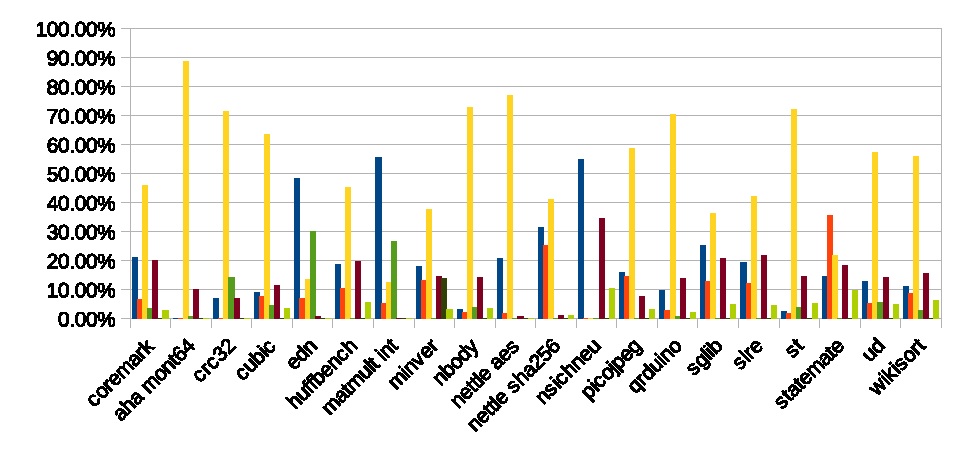
\includegraphics[width=\textwidth]{img/graph/overall_inst_dist}
    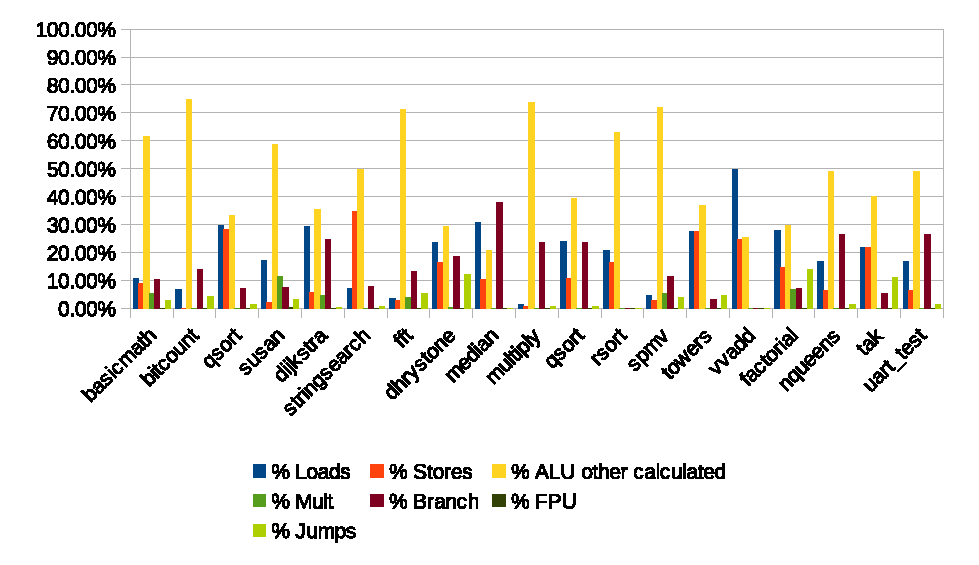
\includegraphics[width=\textwidth]{img/graph/overall_inst_dist2}
    \caption{Overall instruction distribution of all tested benchmarking workloads}
    \label{fig:res/overall/inst}
\end{figure}

\begin{figure}
    \centering
    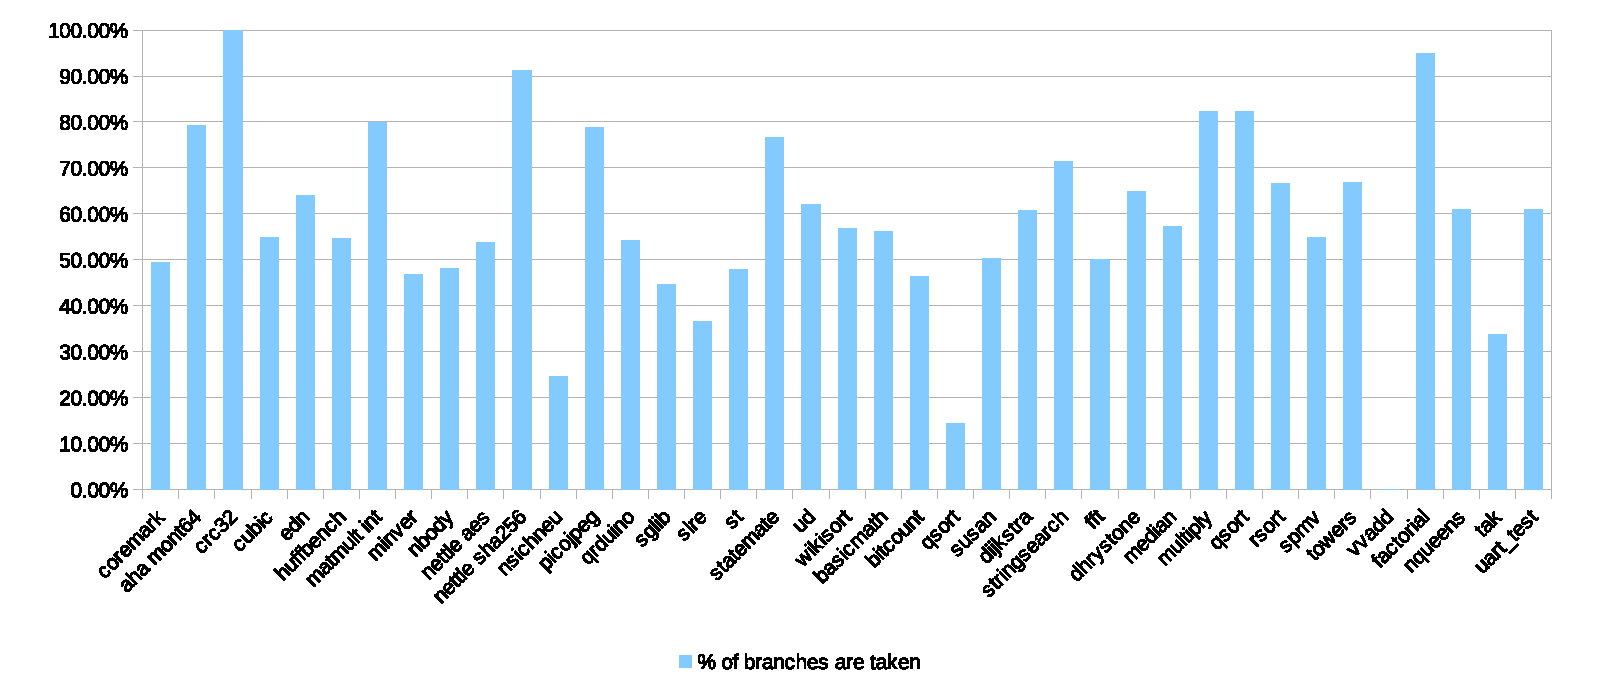
\includegraphics[width=\textwidth]{img/graph/overall_branch_tk.eps}
    \caption{Overall branch taken behavior of all tested benchmarking workloads}
    \label{fig:res/overall/branch_tk}
\end{figure}

\begin{figure}
    \centering
    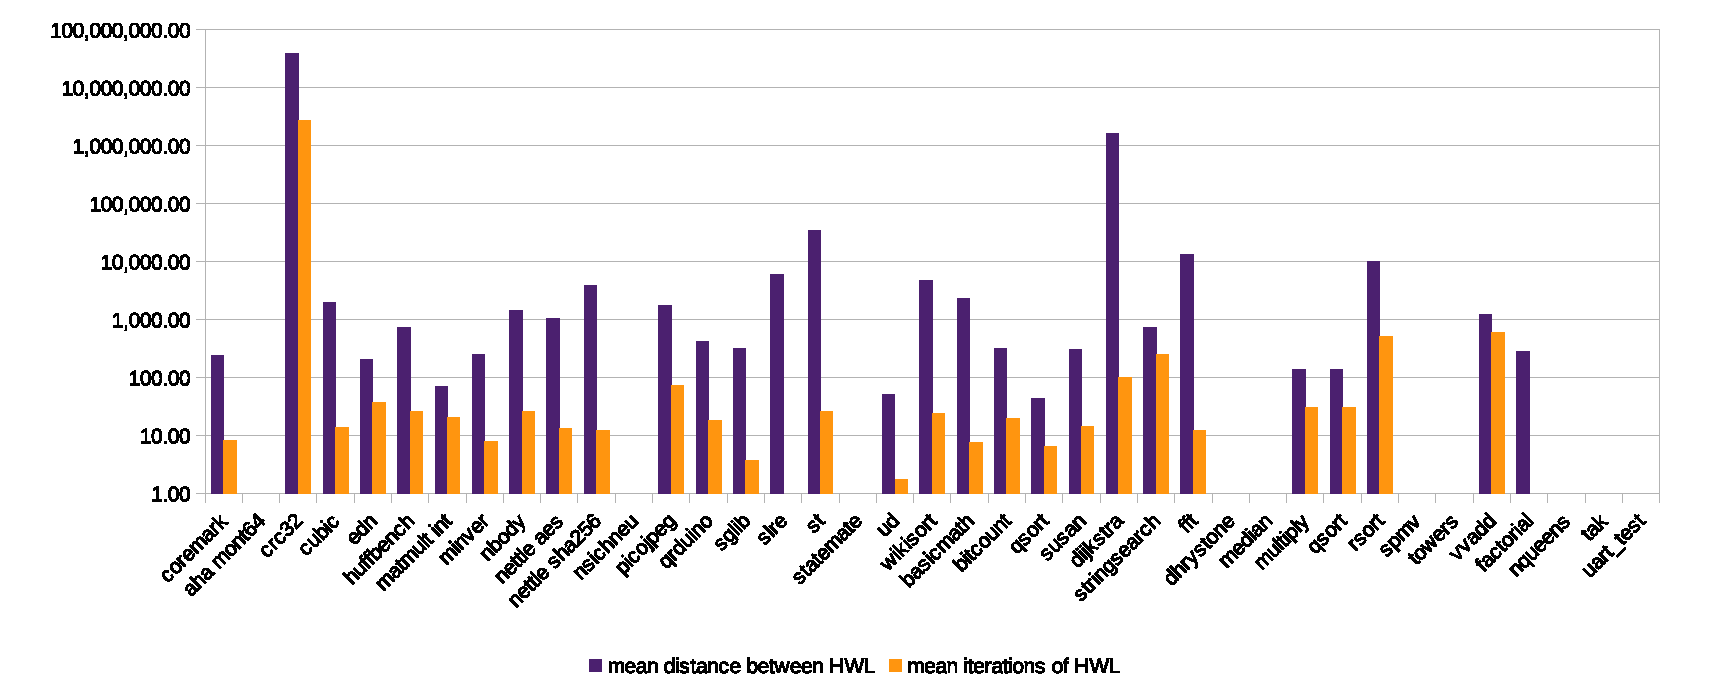
\includegraphics[width=\textwidth]{img/graph/overall_hwl.eps}
    \caption{Overall hardware loop behavior of all tested benchmarking workloads}
    \label{fig:res/overall/hwl}
\end{figure}

\begin{figure}
    \centering
    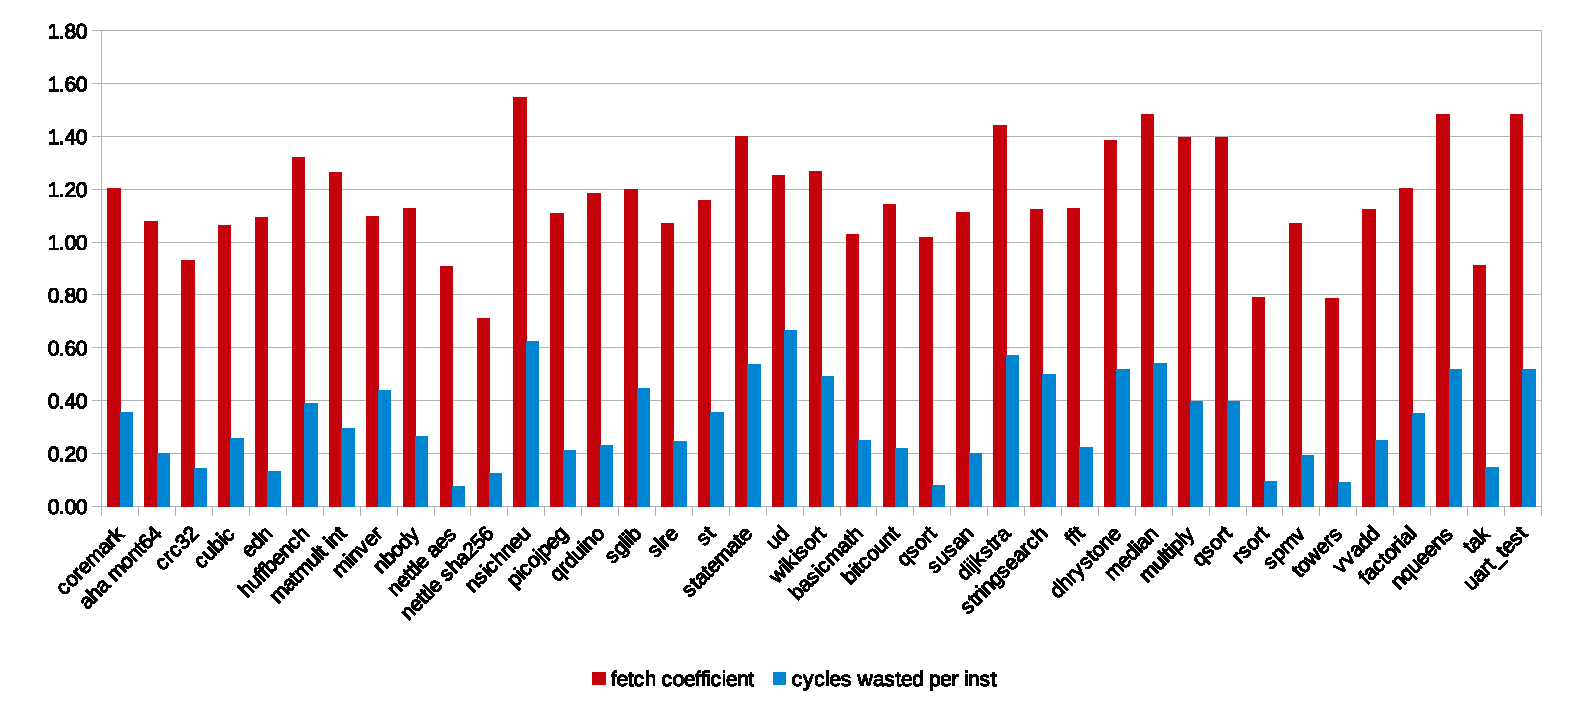
\includegraphics[width=\textwidth]{img/graph/overall_fetch_waste.eps}
    \caption{Overall load coefficient and cycles wasted per instruction of all tested benchmarking workloads}
    \label{fig:res/overall/fetch_waste}
\end{figure}

%% Dhrystone
\begin{figure}
    \centering
    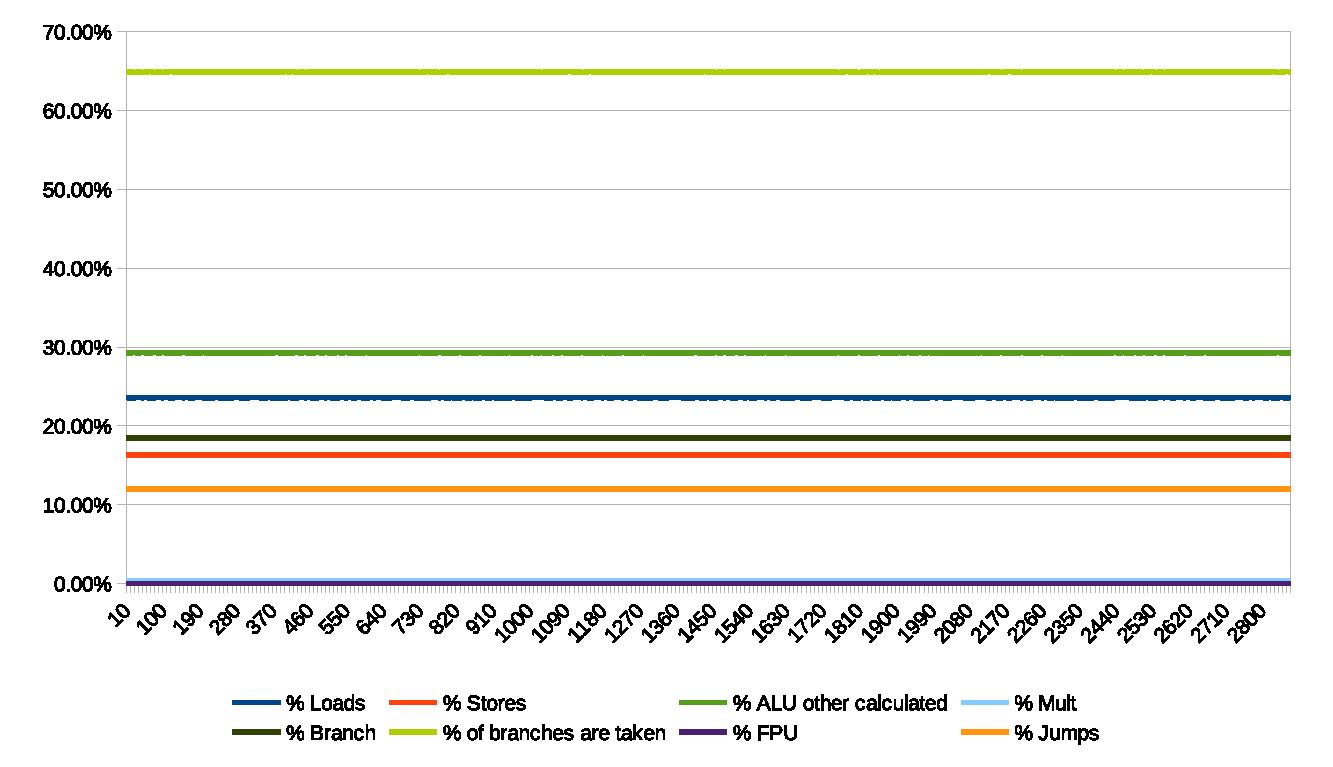
\includegraphics[width=\textwidth]{img/graph/riscv/dhrystone_inst.eps}
    \caption{Instruction distribution over time of Dhrystone (Time in ms)}
    \label{fig:res/dhrystone/inst}
\end{figure}

\begin{figure}
    \centering
    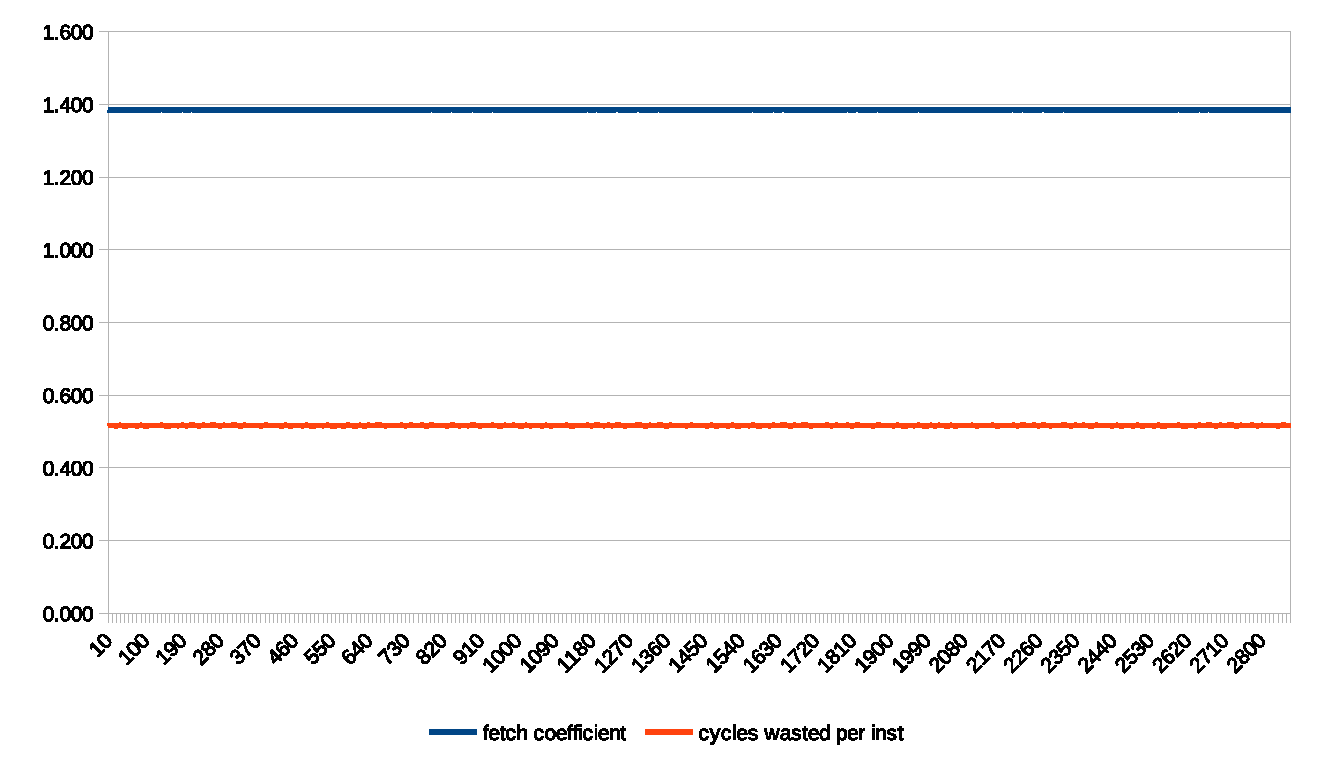
\includegraphics[width=\textwidth]{img/graph/riscv/dhrystone_fetch_waste.eps}
    \caption{Fetch coefficient and cycles wasted per instruction over time of Dhrystone (Time in ms)}
    \label{fig:res/dhrystone/fetch_waste}
\end{figure}

%% bitcount
\begin{figure}
    \centering
    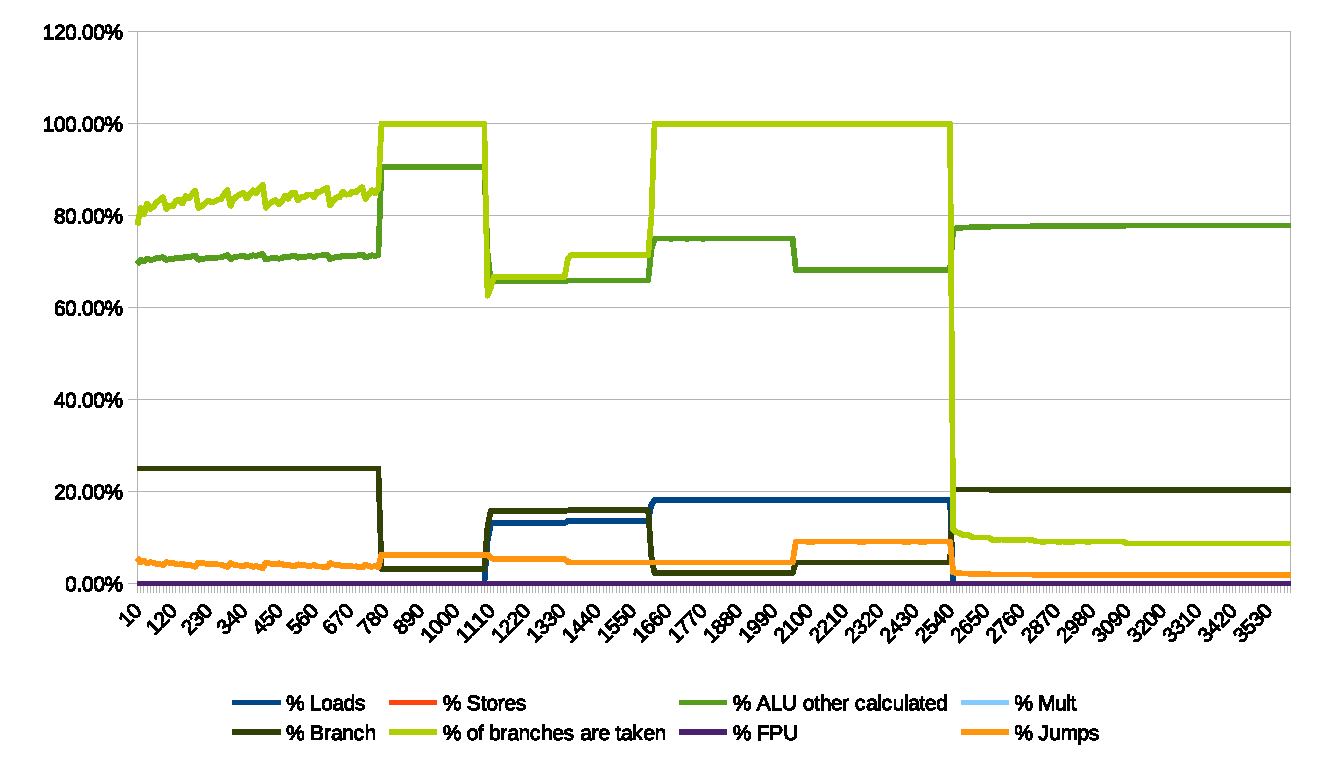
\includegraphics[width=\textwidth]{img/graph/mibench/bitcount_inst.eps}
    \caption{Instruction distribution over time of \texttt{bitcount} (Time in ms)}
    \label{fig:res/bitcount/inst}
\end{figure}

\begin{figure}
    \centering
    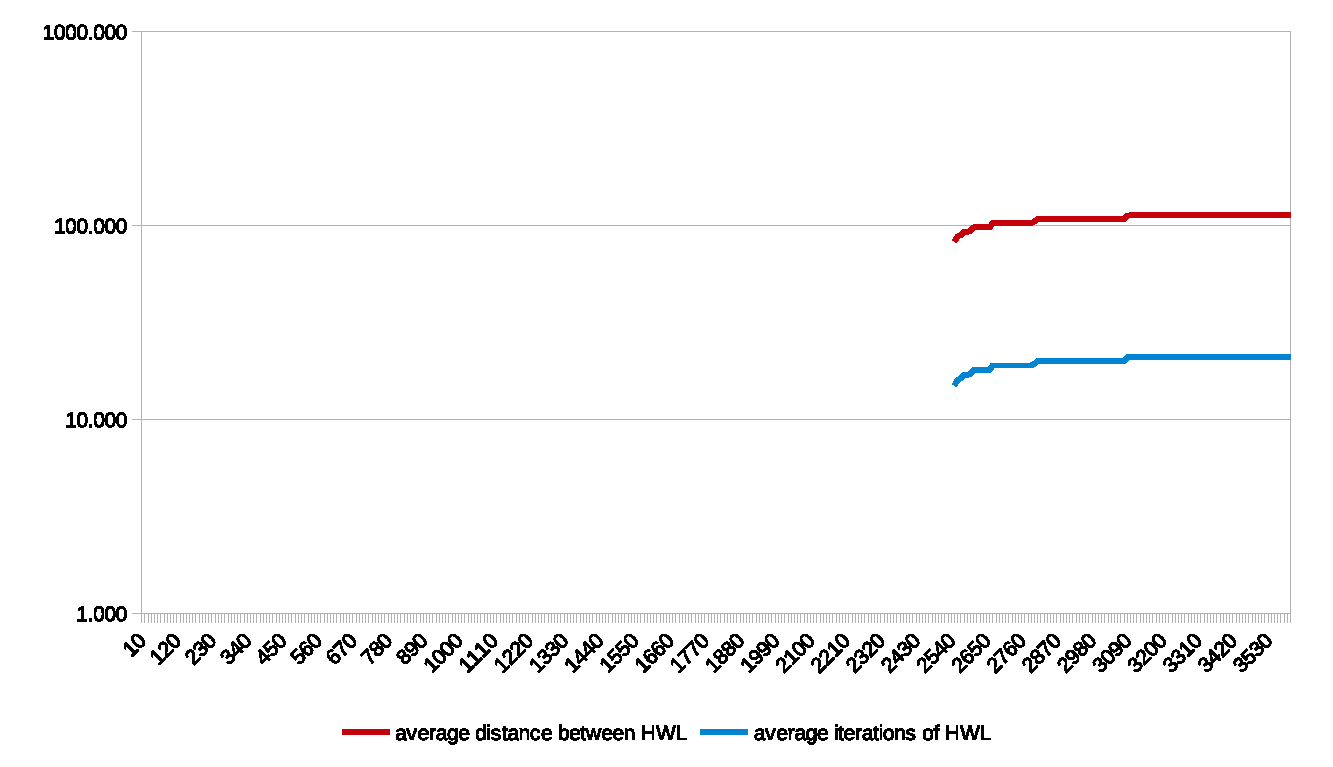
\includegraphics[width=\textwidth]{img/graph/mibench/bitcount_hwl.eps}
    \caption{Hardware loop behavior over time of \texttt{bitcount} (Time in ms)}
    \label{fig:res/bitcount/hwl}
\end{figure}

\begin{figure}
    \centering
    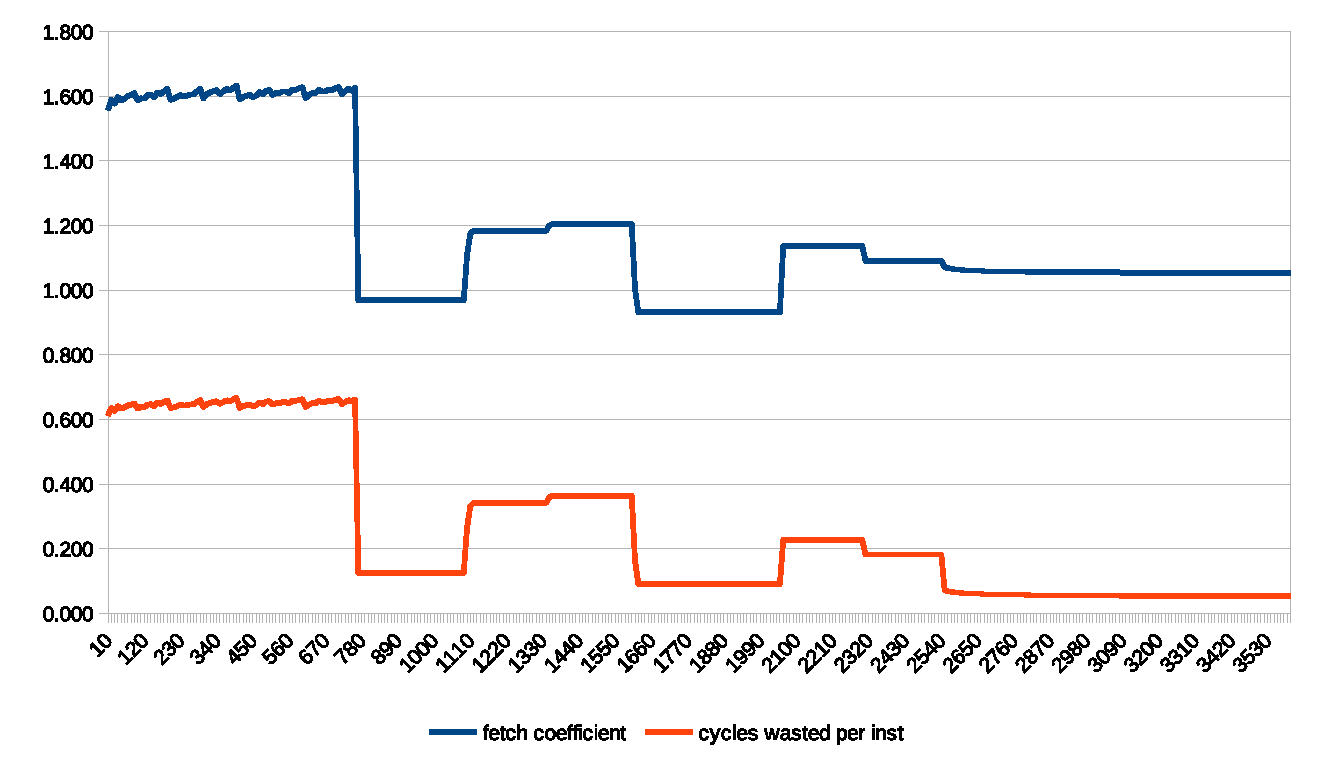
\includegraphics[width=\textwidth]{img/graph/mibench/bitcount_fetch_waste.eps}
    \caption{Fetch coefficient and cycles wasted per instruction over time of \texttt{bitcount} (Time in ms)}
    \label{fig:res/bitcount/fetch_waste}
\end{figure}

%% Coremark
\begin{figure}
    \centering
    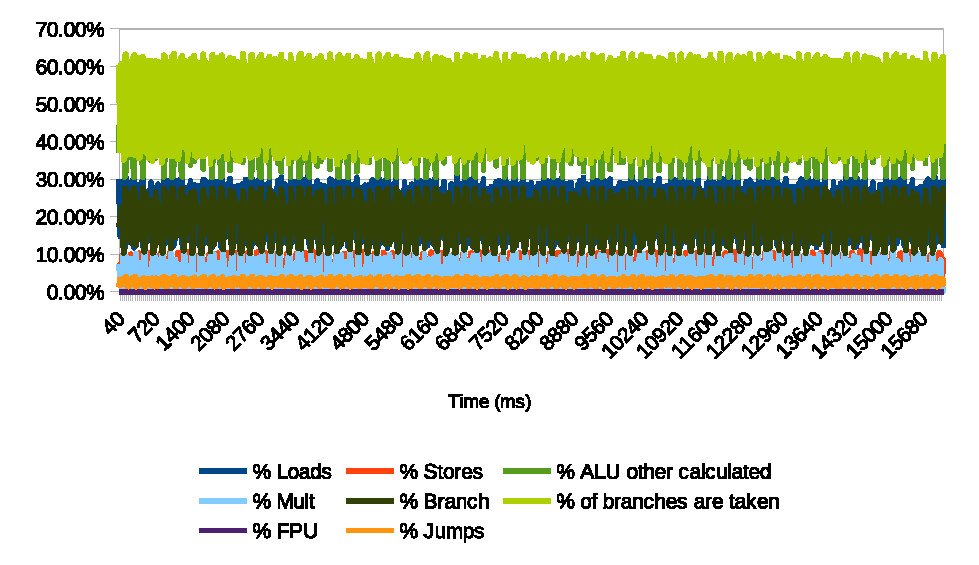
\includegraphics[width=\textwidth]{img/graph/coremark/coremark_inst.eps}
    \caption{Instruction distribution over time of Coremark (Time in ms)}
    \label{fig:res/coremark/inst}
\end{figure}

\begin{figure}
    \centering
    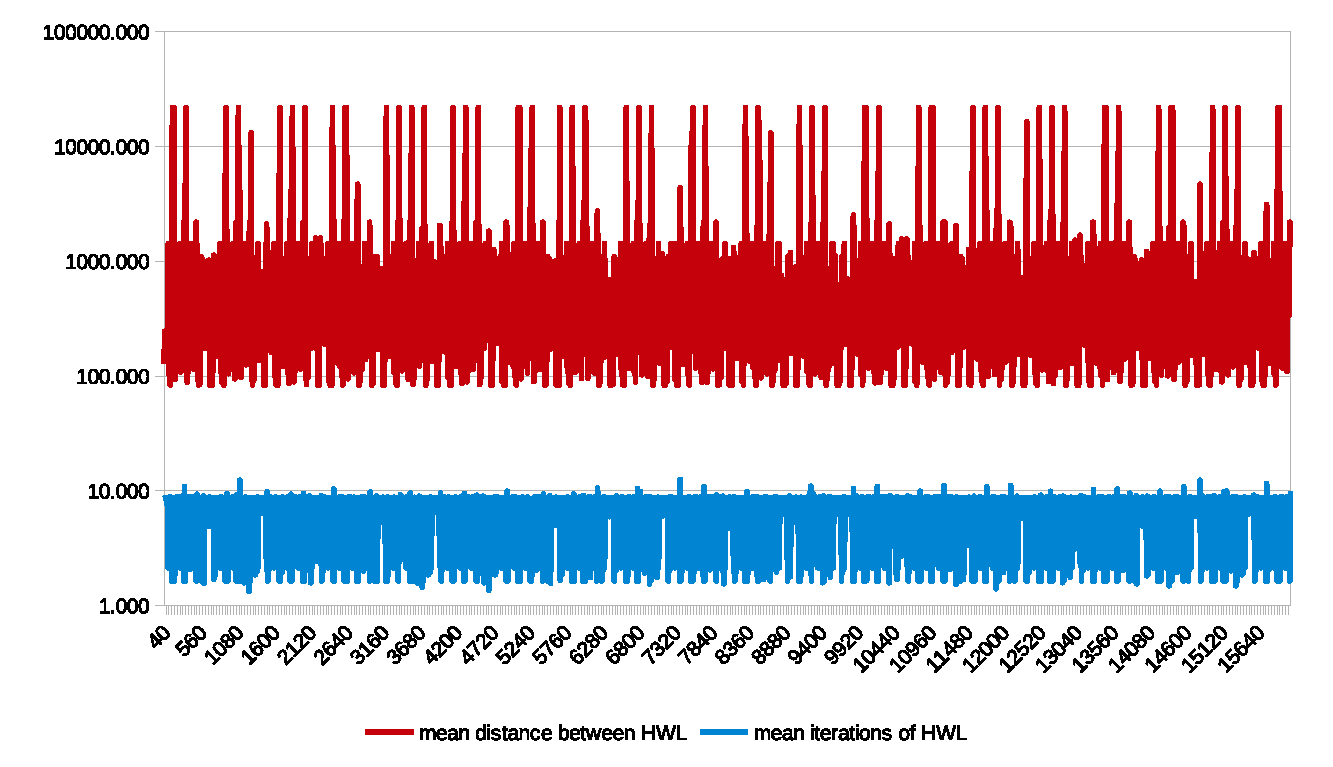
\includegraphics[width=\textwidth]{img/graph/coremark/coremark_hwl.eps}
    \caption{Hardware loop behavior over time of Coremark (Time in ms)}
    \label{fig:res/coremark/hwl}
\end{figure}

\begin{figure}
    \centering
    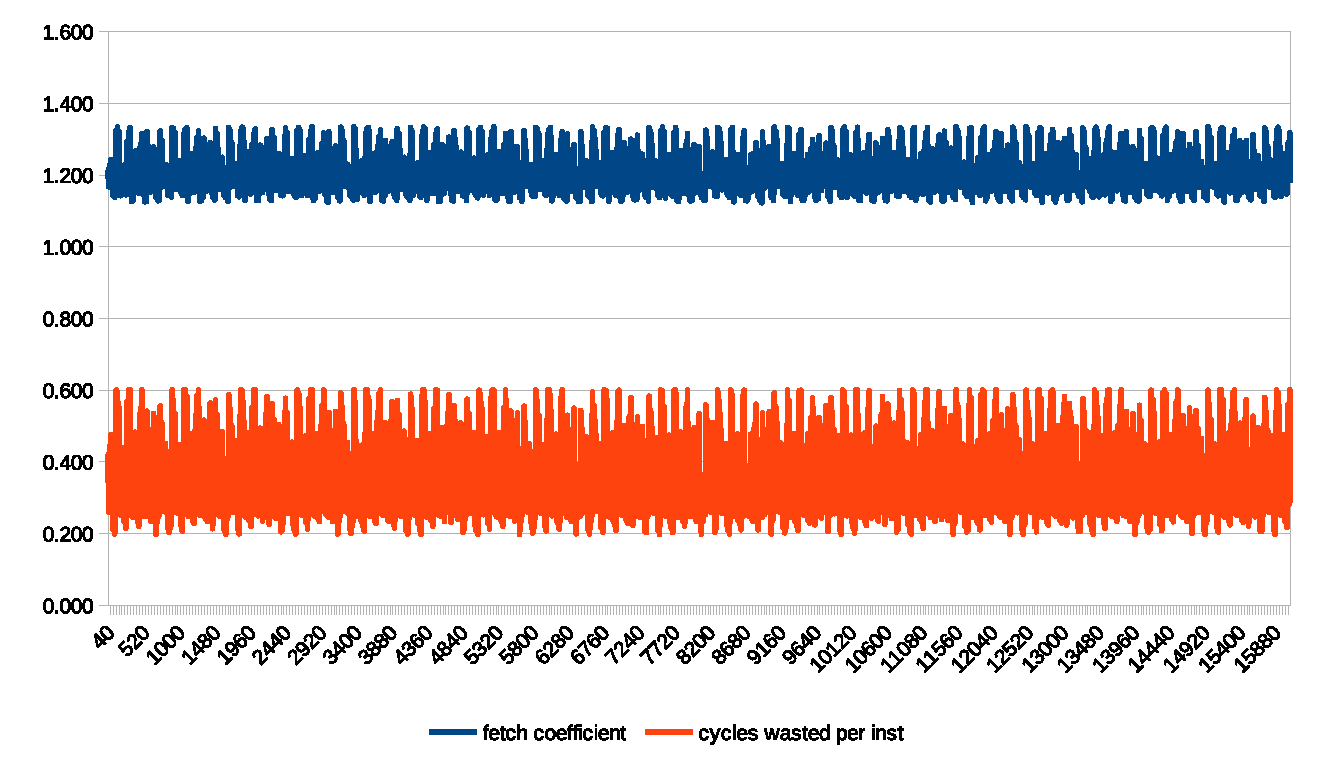
\includegraphics[width=\textwidth]{img/graph/coremark/coremark_fetch_waste.eps}
    \caption{Fetch coefficient and cycles wasted per instruction over time of Coremark (Time in ms)}
    \label{fig:res/coremark/fetch_waste}
\end{figure}

%% sglib
\begin{figure}
    \centering
    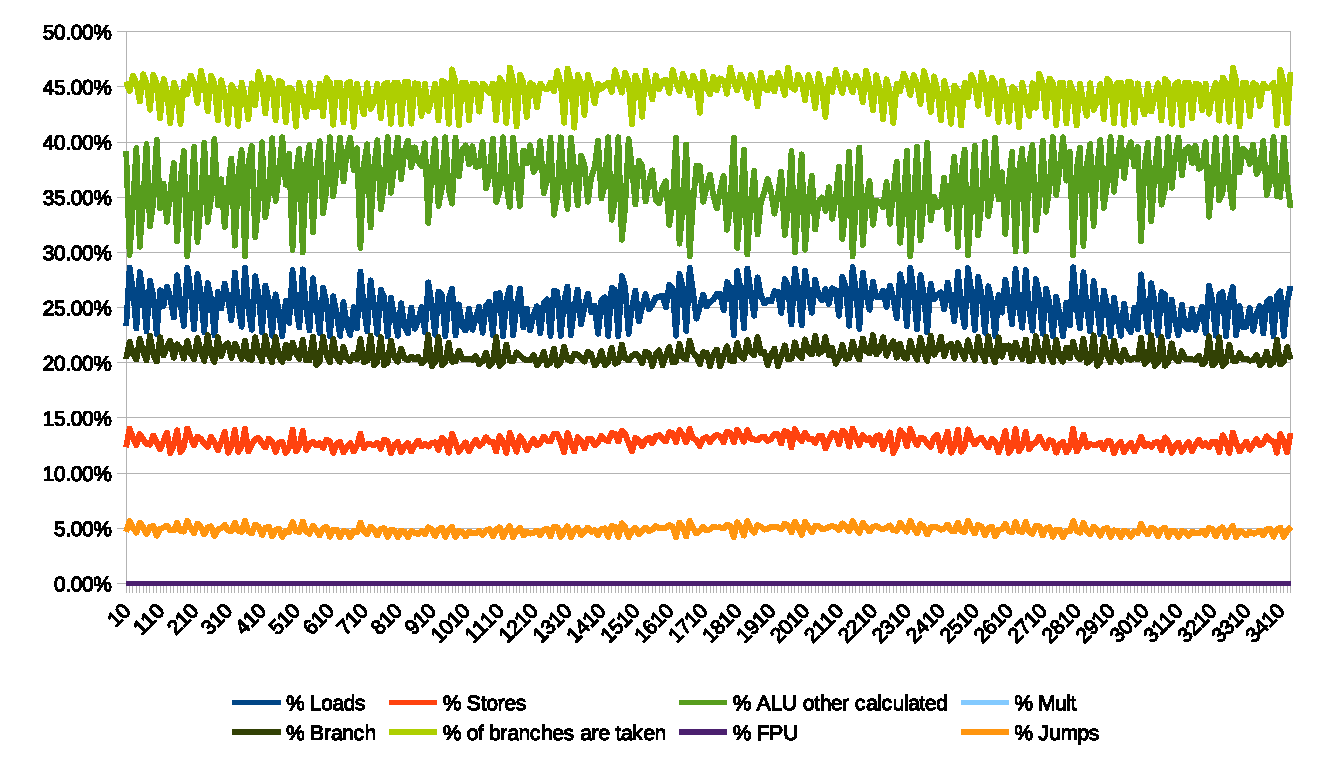
\includegraphics[width=\textwidth]{img/graph/embench/sglib-combined_inst.eps}
    \caption{Instruction distribution over time of \texttt{sglib-combined} (Time in ms)}
    \label{fig:res/sglib/inst}
\end{figure}

\begin{figure}
    \centering
    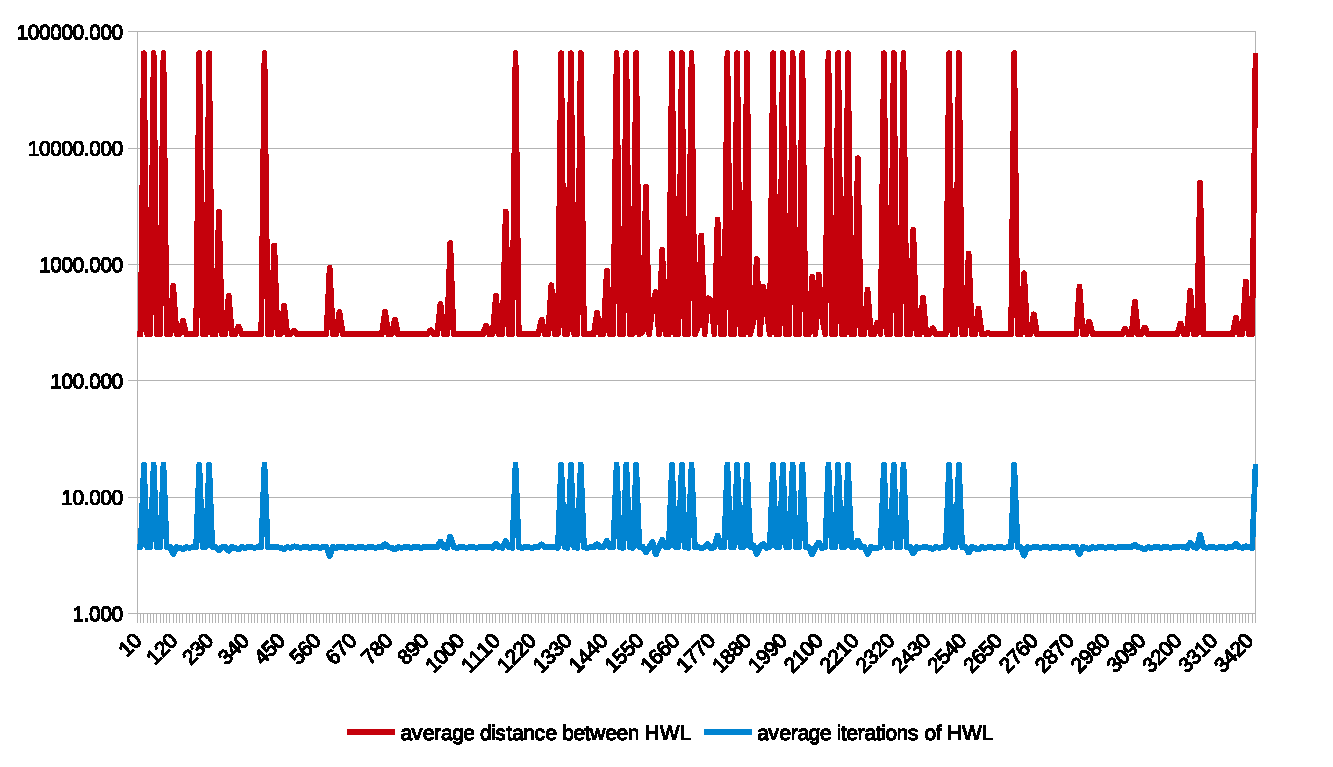
\includegraphics[width=\textwidth]{img/graph/embench/sglib-combined_hwl.eps}
    \caption{Hardware loop behavior over time of \texttt{sglib-combined} (Time in ms)}
    \label{fig:res/sglib/hwl}
\end{figure}

\begin{figure}
    \centering
    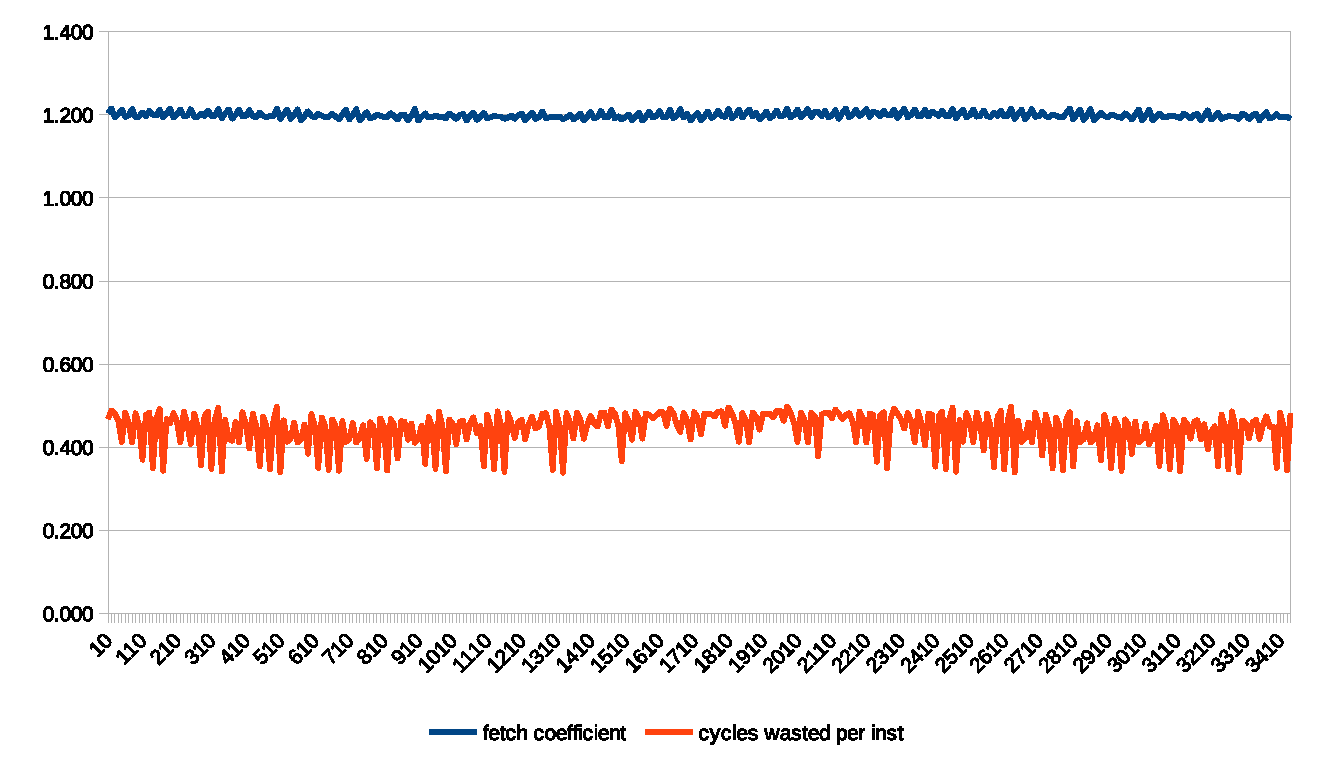
\includegraphics[width=\textwidth]{img/graph/embench/sglib-combined_fetch_waste.eps}
    \caption{Fetch coefficient and cycles wasted per instruction over time of \texttt{sglib-combined} (Time in ms)}
    \label{fig:res/sglib/fetch_waste}
\end{figure}

\section{Metric correlation}
    \label{sec:res/corr}
We calculated the Pearson's correlation coefficient of the different metrics collected in order to gauge metric interdependence. A coefficient closer to 0 is desired, as it indicates little correlation. A metric is intended to represent a single subsystem in the core and each subsystem is mean to be represented by a single metric. More correlation means more bias towards one particular subsystem in the data. For this calculation, we excluded benchmarks \texttt{factorial}, \texttt{nqueens}, \texttt{tak}, and \texttt{uart\_test} due to their very short length. Table \ref{tab:res/corr/coeff} shows the correlation coefficient between metrics. We see moderate correlation with the mean being about 0.25. 

There are outliers however. The most definite example is the correlation between the mean distance between \ac{HWL} initialization and mean \ac{HWL} iteration count as seen in Figure \ref{fig:res/overall/hwl}. Workloads which use \acp{HWL} more often seem to strongly prefer more iterations, while workloads with more distance between \acp{HWL} favor less iterations. RI5CY provides infrastructure for two nested \texttt{for}-loops, this phenomenon in the data could be generated by \texttt{for}-loop heavy programs utilizing \acp{HWL} deeper down in the program. Pearson's correlation coefficient on its own is also not sufficient to identify dependent and independent variables. Further study would be needed to identify the exact cause of this effect. 

We also see a very strong correlation between the fetch coefficient and the cycles wasted. This has to be expected as more fetches require more accesses to higher level memory systems which in turn cause more cycles being wasted. Lastly, we found strong correlation between the share of branching instructions and the fetch coefficient. While this isn't surprising given most workloads seem to favor \emph{branches taken} (as suppose to \emph{branches not taken} implemented by RI5CY), more branching instructions directly means more instructions fetched. What was surprising was the rather small correlation between the fetch coefficient and the share of taken branches.

\begin{table}
    \centering
    \resizebox{\textwidth}{!}{%
    \begin{tabular}{l|SSSSSSSSS}
                        & \% Branch     & {\% br. taken}    & \% FPU    & \% Jumps  & {mean dist.}  & {mean it.}    & {fetch coeff.}    & {cycles wasted /} \\
                        &               &                   &           &           & HWL           & HWL           &                   & instruction       \\
        \hline
        \% Mult         & -0.37         &  0.24             & -0.09     & -0.27     &  0.26         &  0.26         & -0.04             & -0.19             \\ \hline
        \% Branch       &               & -0.12             &  0.02     &  0.39     & -0.10         & -0.11         &  0.79             &  0.72             \\ \hline
        \% br. taken    &               &                   & -0.10     & -0.20     &  0.36         &  0.36         & -0.11             & -0.03             \\ \hline
        \% FPU          &               &                   &           & -0.01     & -0.03         & -0.03         & -0.05             &  0.13             \\ \hline
        \% Jumps        &               &                   &           &           & -0.19         & -0.18         &  0.37             &  0.45             \\ \hline
        mean dist. HWL  &               &                   &           &           &               &  1.00         & -0.19             & -0.17             \\ \hline
        mean it. HWL    &               &                   &           &           &               &               & -0.20             & -0.18             \\ \hline
        fetch coeff.    &               &                   &           &           &               &               &                   &  0.82             \\
    \end{tabular}}
    \caption{Pearson's correlation coefficient between metrics}
    \label{tab:res/corr/coeff}
\end{table}

% Render bibliograhy and acronyms if rendered standalone
\isstandalone
\bibliographystyle{IEEEtran}
\bibliography{bibliography}
\subfile{abbreviations.tex}
\fi

\end{document} 
